%%%%%%%%%%%%%%%%%%%%%%%%%%%%%%%%%%%%%%%%%%
%%%%%%%%%%%%%%%% Imagenes %%%%%%%%%%%%%%%%
%%%%%%%%%%%%%%%%%%%%%%%%%%%%%%%%%%%%%%%%%%

%Author: Antonio Avilix
%Year:2020

%%%%%%%%Preambulo%%%%%%%%

\documentclass{article}
\usepackage[utf8]{inputenc}
\usepackage[spanish]{babel}
\usepackage{amsmath, amssymb, amsfonts}
\usepackage{graphicx}
\usepackage{subcaption}
\usepackage{wrapfig}
\usepackage{lipsum}
\graphicspath{{images/}}

\title{Imagenes}
\author{Toño Avilix}
\date{Sin Fecha}

\begin{document}

\maketitle


\includegraphics{dog1.png}

\includegraphics[scale=1.5, angle=60]{dog1.png}
\begin{figure}[h]
    \centering
    
\includegraphics{dog2.jpg}
    \caption{Perro}
    \label{fig:perro1}
\end{figure}
\begin{figure}[h!]
    \centering
    \begin{subfigure}[b]{0.47\linewidth}
        
\includegraphics[width=\linewidth]{dog1.png}
        \caption{Perro1}
        \label{figs:perro1}
    \end{subfigure}
    \begin{subfigure}[b]{0.47\linewidth}
        
\includegraphics[width=\linewidth]{dog2.jpg}
        \caption{Perro2}
        \label{figs:perro2}
    \end{subfigure}  
    \caption{Mis perros}
    \label{fig:misperros} 
\end{figure}

\lipsum[1]
\begin{wrapfigure}{r}{0.4\linewidth}
    \centering
    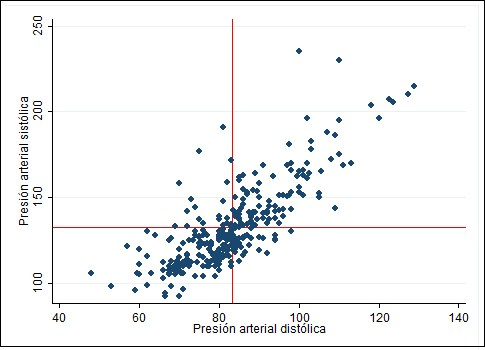
\includegraphics[width=0.4\textwidth]{grafica1.jpg}
    \caption{Grafica}
    \label{fig:myfig}
\end{wrapfigure}
\lipsum[1]

\end{document}